\begin{figure}[h]
    \centering
    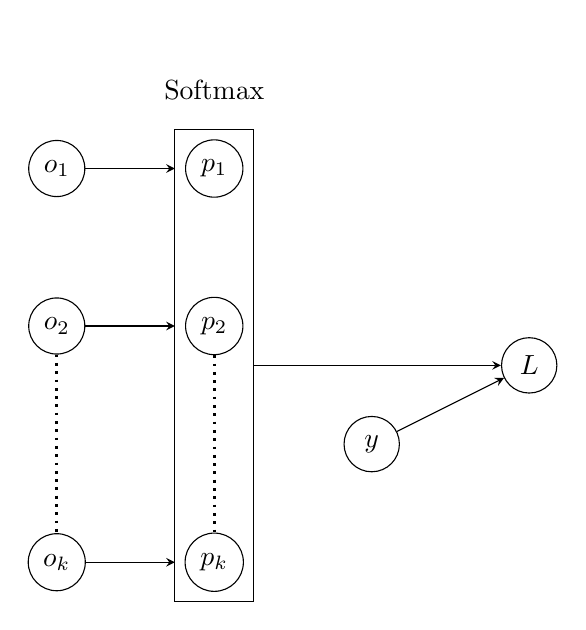
\begin{tikzpicture}[
        node/.style=draw, circle, minimum width=2em,
        forward/.style=->, >=stealth,
        scale=2
    ]
        \node[node] (o1) at (0, 0) {$o_1$};
        \node[node] (o2) at (0, -1) {$o_2$};
        \node[node] (ok) at (0, -2.5) {$o_k$};
        \draw[dotted, line width=1pt] (o2) -- (ok);
        \node[node] (p1) at (1, 0) {$p_1$};
        \node[node] (p2) at (1, -1) {$p_2$};
        \node[node] (pk) at (1, -2.5) {$p_k$};
        \draw[dotted, line width=1pt] (p2) -- (pk);
        \node[] (sm) at (1, 0.5) {Softmax};
        \draw (0.75, 0.25) rectangle (1.25, -2.75);
        \node[node] (y) at (2, -1.75) {$y$};
        \node[node] (l) at (3, -1.25) {$L$};
        \draw[forward] (o1) -- (0.75, 0);
        \draw[forward] (o2) -- (0.75, -1);
        \draw[forward] (ok) -- (0.75, -2.5);
        \draw[forward] (y) -- (l);
        \draw[forward] (1.25, -1.25) -- (l);
    \end{tikzpicture}
    \caption{Softmax computation graph for gradient boosted tree output}
\end{figure}
